\documentclass{article}
\usepackage[utf8]{inputenc}
\usepackage{graphicx}
\usepackage{wrapfig}

\title{Application of Diode\\ ELP101\\Lab Report 5}
\author{Aditya Agrawal\\2021AM10198\\GROUP 29}
\date{May 26, 2022}
\begin{document}

\maketitle
\tableofcontents
\newpage

\section{Diode Half Wave Rectifier}
\subsection{Aim}
To investigate the characteristic of diode half wave rectifier.
\subsection{Apparatus Required}
\begin{enumerate}
    \item Electrolytic Capacitor
    \item Function Generator (0 – 3 MHz)
    \item Breadboard and Jumpers
    \item Multimeter and Resistors
    \item Silicon Diode
    \item Digital Storage Oscilloscope (DSO1052B)
\end{enumerate}
\subsection{Theory}
A rectifier is an electrical component that converts alternating current (AC), which periodically reverses direction, to unidirectional direct current (DC). This procedure is referred to as rectification. Rectifiers have numerous applications, but they are most commonly found in DC power supplies and high-voltage DC power transmission systems.\par
\begin{figure}[h!]
    \centering
    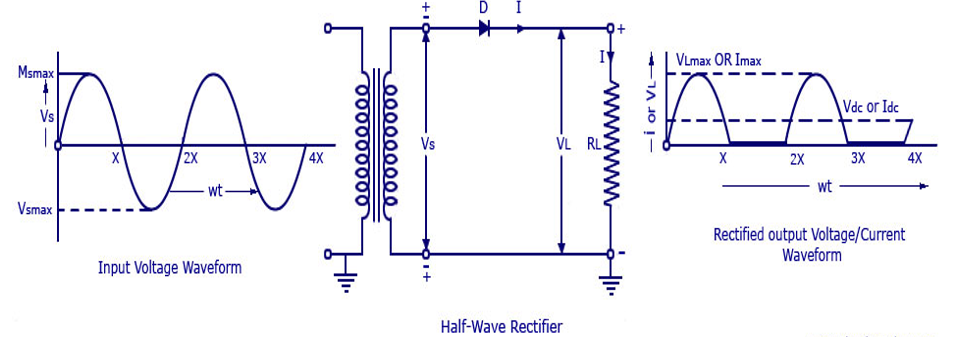
\includegraphics[width=1\textwidth]{pic1.png}
    \caption{Half Wave Rectifier}
\end{figure}
A simple Half Wave Rectifier consists of a single pn junction diode in series with the load resistor. Figure depicts the half-wave rectifier circuit using a semiconductor diode (D) and a load resistance (RL), but no smoothing filter. In series with the secondary of the transformer and the load resistance RL is the diode. The transformer's primary winding is connected to the ac supply mains.\par
During the positive half-cycles of the input ac voltage, or when the upper end of the secondary winding is positive with respect to its lower end, the diode is forward biased and conducts current. If the forward resistance of the diode is assumed to be zero (in practise, a small resistance exists), the input voltage during the positive half-cycles is applied directly to the load resistance RL, making its upper end positive relative to its lower end. The wave forms of the output current and voltage are identical to the waveform of the input ac voltage.\par
During the negative half cycles of the input ac voltage, that is, when the lower end of the secondary winding is positive relative to its upper end, the diode is reverse biased and therefore does not conduct. Consequently, during the negative half cycles of the input ac voltage, the load current and voltage remain at zero. The magnitude of the reverse current is so small that it is disregarded. Consequently, during the negative half cycles, no power is supplied to the load.

\subsection{Breadboard Setup}
\begin{figure}[h!]
\centering
    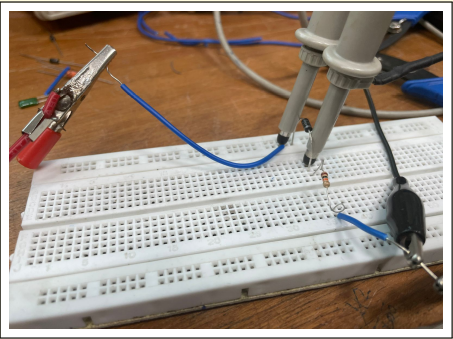
\includegraphics[width=0.5\textwidth]{pic2.png}
    \caption{Circuit with R=10k$\Omega$}
    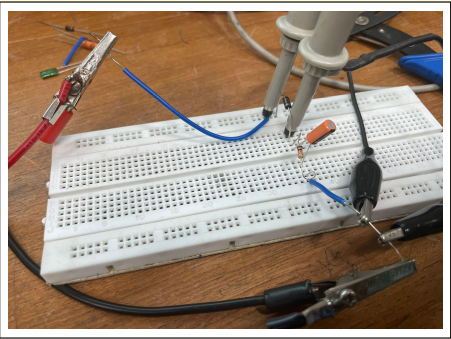
\includegraphics[width=0.5\textwidth]{pic3.png}
    \caption{Circuit with Electrolytic Capacitor in
Parallel}
\end{figure}
\newpage
\subsection{DSO Images}

\begin{figure}[h]
\centering
    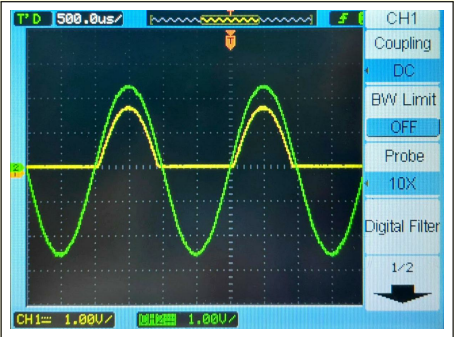
\includegraphics[width=0.5\textwidth]{pic4.png}
    \caption{Voltage with Resistor}
    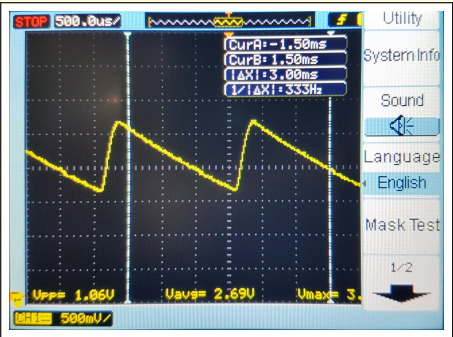
\includegraphics[width=0.5\textwidth]{pic5.png}
    \caption{Voltage with Resistor and Capacitor}
\end{figure}
\subsection{Observations}
\begin{center}
\begin{tabular}{|c|c|c|c|}
\hline
    $V_{0}$=5V & $V_{Input}$(V) & $V_{Output}$(V) & $V_{Output}$ with Capacitor(V) \\
    \hline
    $V_{PP}$ & 4.88 & 1.76 & 0.53\\
    $V_{avg}$ & -58.3 & 517 & 1.34 \\
\hline
\end{tabular}\vspace{3mm}
\begin{tabular}{|c|c|c|c|}
\hline
    $V_{0}$=0.5V & $V_{Input}$(mV) & $V_{Output}$(mV) & $V_{Output}$ with Capacitor(mV) \\
    \hline
    $V_{PP}$ & 480 & 126 & 23\\
    $V_{avg}$ & -9.87 & 49.93 & 37 \\
\hline
\end{tabular}
\end{center}
\subsection{Conclusion}
Hence we see the output waveforms for a Half-wave Rectifier in the case of a simple resistor and when capacitor smoothing happens.
\newpage
\section{Diode Clipping Circuit}
\subsection{Aim}
To investigate the characteristic of diode clipping circuit.
\subsection{Apparatus Required}
\begin{enumerate}
    \item Function Generator (0 – 3 MHz)
    \item Breadboard and Jumpers
    \item Multimeter and Resistors
    \item Silicon Diode
    \item Digital Storage Oscilloscope (DSO1052B)
    \item DC Power Supply
\end{enumerate}
\subsection{Theory}
This clipping of the input signal produces an output waveform that resembles a flattened version of the input. For example, the half-wave rectifier is a clipper circuit, since all voltages below zero are eliminated.\par
\begin{figure}[h!]
    \centering
    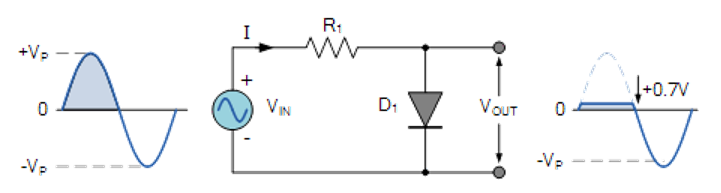
\includegraphics[width=1\textwidth]{pic6.png}
    \caption{Clipping circuit diagram with input and output waveforms with forward biasing of diode}
\end{figure}
In this diode clipping circuit, the diode is forward biased during the sinusoidal input wave-form's positive half cycle. For the diode to become forward biased, the magnitude of its input voltage must exceed +0.7 volts. When this occurs, the diode conducts and maintains a constant voltage of 0.7V across itself until the sinusoidal waveform falls below this value. Thus, the output voltage measured across the diode during the positive half cycle can never exceed 0.7 volts.\par
During the negative half cycle, the diode is reverse biased, preventing current flow through itself. As a result, the negative half of the sinusoidal voltage is unaffected and passes through unaltered to the load. A positive clipper circuit consists of a diode that restricts the positive portion of the input waveform.\par
\begin{figure}[h!]
    \centering
    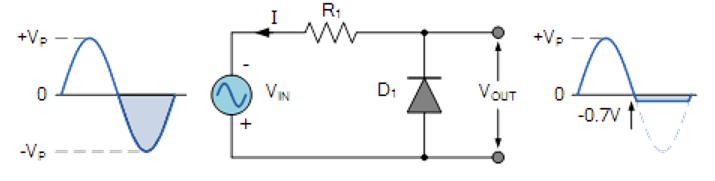
\includegraphics[width=1\textwidth]{pic7.png}
    \caption{Clipping circuit diagram with input and output waveforms with forward biasing of diode}
\end{figure}
By modifying biasing, we can alter the clipping timing in the graph. Similarly, by placing two diodes in parallel in the circuit, clipping can be enabled at all times in the waveform.\\
\textbf{Diode and Source Polarities are considered +ve as per the circuit on the right.}
\subsection{Breadboard Setup}
\begin{figure}[h!]
\centering
    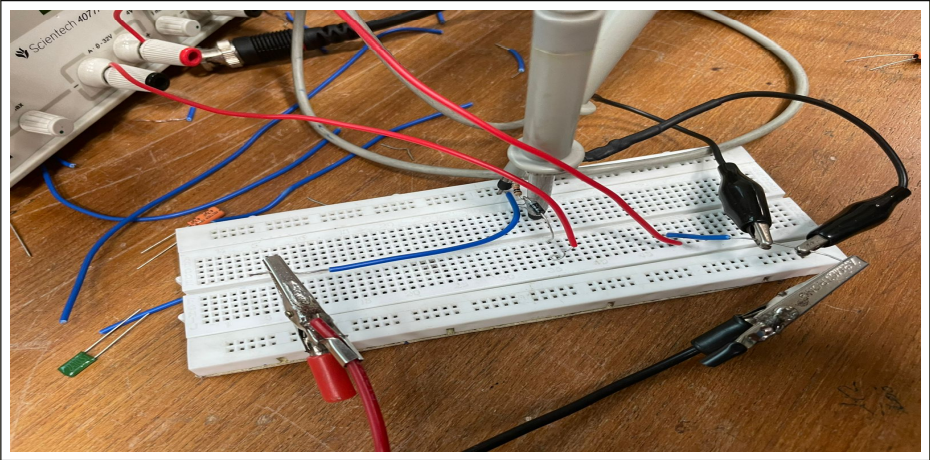
\includegraphics[width=0.5\textwidth]{pic8.png}
    \caption{Circuit with R=10k$\Omega$ and V=2V}
\end{figure}
\subsection{DSO Images}
\begin{center}
    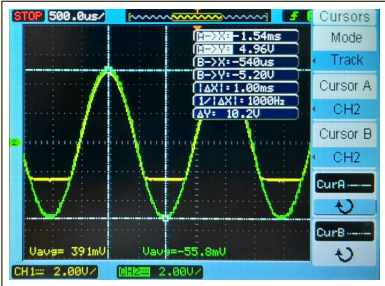
\includegraphics[width=0.4\textwidth]{pic9.png}
    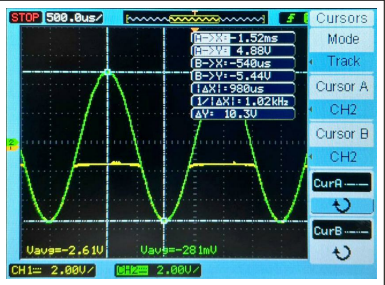
\includegraphics[width=0.4\textwidth]{pic10.png}\\
    D:+ S:+ \hspace{30mm}D:- S:+\\
    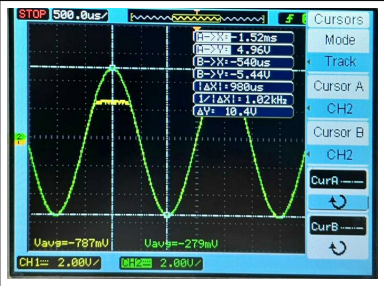
\includegraphics[width=0.4\textwidth]{pic11.png}
    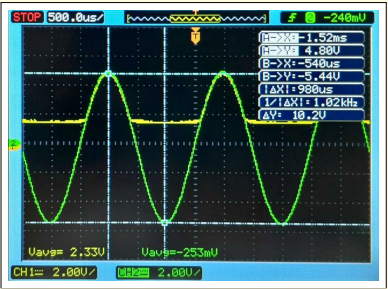
\includegraphics[width=0.4\textwidth]{pic12.png}\\
    D:- S:- \hspace{30mm}D:+ S:-\\
\end{center}
\subsection{Observations}
\begin{center}
\begin{tabular}{|c|c|c|c|c|}
\hline
    Signal & $Input_{PP}$(V) & $Input_{avg}$(mV) & $Output_{PP}(V)$ & $Output_{avg}$(mV) \\
    \hline
    D:+ S:+ & 10.2 & -55.8 & 7.36 & 391\\
    D:- S:+ & 10.3 & -281 & 3.92 & -2610 \\
    D:- S:- & 10.4 & -279 & 7.92 & -787\\
    D:+ S:- & 10.2 & -253 & 3.36 & 2330\\
\hline
\end{tabular}
\end{center}
\subsection{Conclusion}
Hence we see the output waveforms for a Clipper circuit and observe the changes when we reverse the polarities of source or diode.
\newpage
\section{Diode Clamping Circuit}
\subsection{Aim}
To investigate the characteristic of diode clamping circuit.
\subsection{Apparatus Required}
\begin{enumerate}
    \item Function Generator (0 – 3 MHz)
    \item Breadboard and Jumpers
    \item Multimeter and Resistors
    \item Silicon Diode
    \item Digital Storage Oscilloscope (DSO1052B)
    \item DC Power Supply
    \item Non-electrolytic Capacitor
\end{enumerate}
\subsection{Theory}
\begin{wrapfigure}{R}{0.2\textwidth}
    {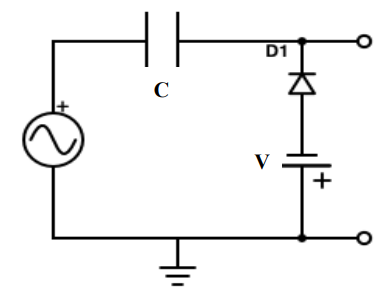
\includegraphics[width=0.25\textwidth]{pic13.png}}
\end{wrapfigure}
A clamper is an electronic circuit that shifts the DC value in order to clamp either the positive or negative peak excursions of a signal to a predetermined value. The clamper does not limit the signal's peak-to-peak excursion; rather, it shifts the entire signal up or down to place the peaks at the reference level. A diode clamp is comprised of a diode and a capacitor that supplies a DC offset from the stored charge.\\
\textbf{Diode and Source Polarities are considered +ve as per the circuit on the right.}
\subsection{Breadboard Setup}
\begin{figure}[h!]
    \centering
    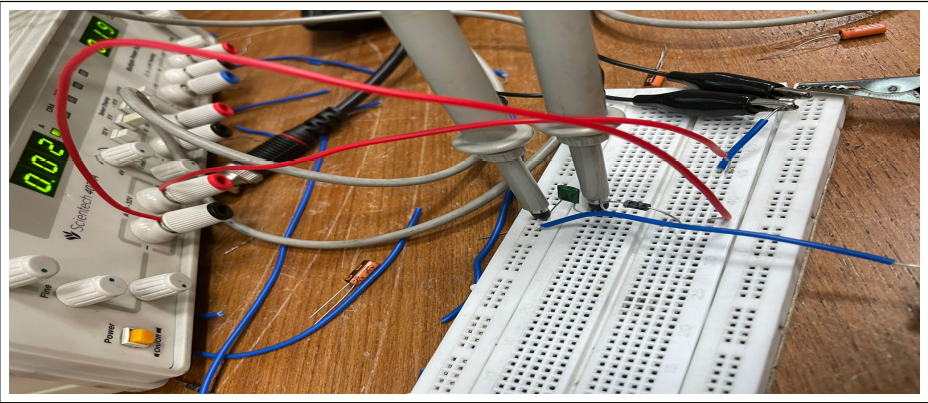
\includegraphics[width=0.7\textwidth]{pic14.png}
    \caption{Circuit with C = 0.01µF and V=2V}
\end{figure}
\subsection{DSO Images}
\begin{center}
    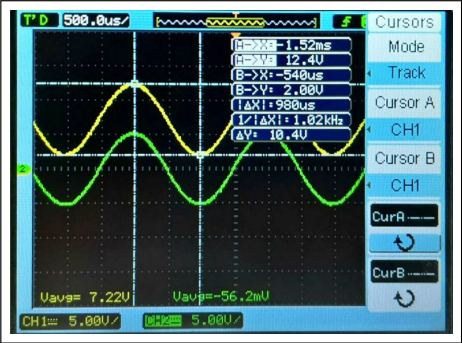
\includegraphics[width=0.4\textwidth]{pic15.png}
    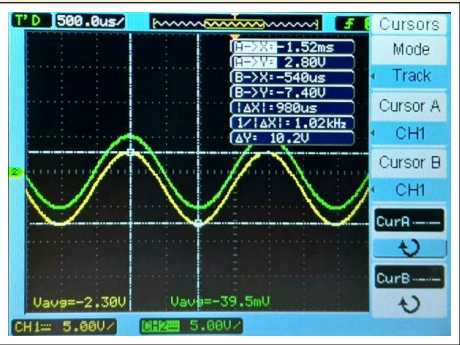
\includegraphics[width=0.4\textwidth]{pic16.png}\\
    D:+ S:+ \hspace{30mm}D:- S:+\\
    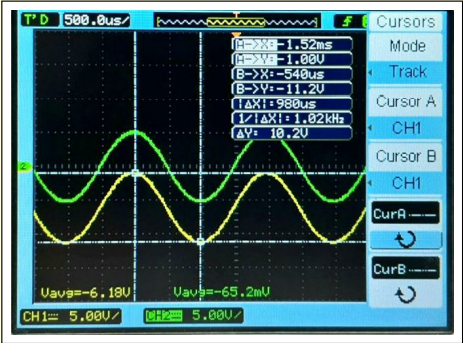
\includegraphics[width=0.4\textwidth]{pic17.png}
    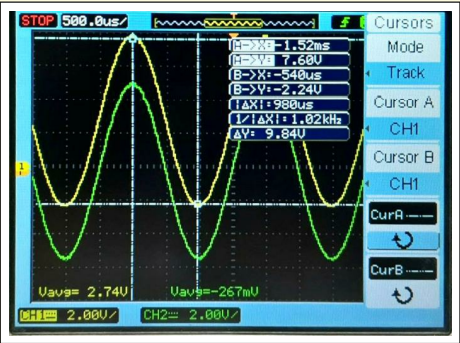
\includegraphics[width=0.4\textwidth]{pic18.png}\\
    D:- S:- \hspace{30mm}D:+ S:-\\
\end{center}
\subsection{Observations}
\begin{center}
\begin{tabular}{|c|c|c|c|c|}
\hline
    Signal & $Input_{PP}$(V) & $Input_{avg}$(mV) & $Output_{PP}(V)$ & $Output_{avg}$(V) \\
    \hline
    D:+ S:+ & 10.2 & -56.2 & 10.4 & 7.22\\
    D:- S:+ & 10.2 & -39.5 & 10.2 & -2.30 \\
    D:- S:- & 10.2 & -65.2 & 10.2 & -6.18\\
    D:+ S:- & 10.2 & -267 & 9.84 & 2.74\\
\hline
\end{tabular}
\end{center}
\subsection{Conclusion}
Hence we see the output waveforms for a Clamper circuit and observe the changes when we reverse the polarities of source or diode.
\newpage
\section{Sources Of Error}
\begin{itemize}
    \item Resistance of wires not taken into account, and also giving rise to inconsistency due to increase in resistance due to heating.
    \item Change in the connections while circuit is closed.
    \item Loose Connections.
    \item Scale of DSO not appropriate for measurements.
\end{itemize}
\section{Precautions}
\begin{itemize}
    \item Make the connections neat and tight.
    \item Wear proper shoes and use insulated tools.
    \item Don’t leave the switch on for long continuous periods of time.
\end{itemize}
\section{Concluding Remarks}
In the preceding experiment, we investigated the use of a diode as a rectifier, in a clipping circuit, and in a clamping circuit. Using a single diode in a circuit produces a half-wave rectifier, which allows only one portion of the current cycle to pass through (positive or negative). The voltage is rectified because the diode prevents the other half of the input wave from passing through.

In a clipping circuit, a diode with a DC Source can be used to clip a portion of the input signal. The polarity of the diode determines which half of the wave signal is clipped, and the DC Source voltage determines the threshold voltage above which the wave signal is clipped (or below). The results were also as expected.

In a clamping circuit, the voltage is shifted by one-half of the peak-to-peak value (depending on the external source) above or below its initial mean value. The DSO screens display the same information.\par
Thus, diodes can successfully rectify, clip, or clamp AC signals.
\end{document}
